%%%%%%%%%%%%%%%%%%%%%%%%%%%%%%%%%%%%%%%%%%%%%%%%%%%%%%%%%%%%%%%
%
% Welcome to Overleaf --- just edit your LaTeX on the left,
% and we'll compile it for you on the right. If you open the
% 'Share' menu, you can invite other users to edit at the same
% time. See www.overleaf.com/learn for more info. Enjoy!
%
%%%%%%%%%%%%%%%%%%%%%%%%%%%%%%%%%%%%%%%%%%%%%%%%%%%%%%%%%%%%%%%

% ===============================================
% MATH 790: Real Analysis           Spring 2022
% hw_template.tex
% ===============================================

% -------------------------------------------------------------------------
% The preamble that follows can be ignored. Go on
% down to the section that says "START HERE" 
% -------------------------------------------------------------------------


% https://www.overleaf.com/latex/templates/proof-template-for-real-analysis/ztkshxkdstfk
\documentclass{article}

\usepackage[margin=1in]{geometry} 
\usepackage{xcolor}
\usepackage{graphicx}
\usepackage{eqparbox}
\usepackage[abbreviations]{foreign}
\usepackage{caption}
\usepackage{natbib}
\setcitestyle{square}
\usepackage{wrapfig}
\usepackage{subcaption}
\usepackage{amsmath,amsthm,amssymb,hyperref}

\renewcommand{\figureautorefname}{Fig.}
%\renewcommand{\tableautorefname}{Tab.}
\renewcommand{\equationautorefname}{Eq.}

\hypersetup{
	colorlinks   = true, %Colours links instead of ugly boxes
	urlcolor     = blue, %Colour for external hyperlinks
	linkcolor    = blue, %Colour of internal links
	citecolor   = red %Colour of citations
}

\newcommand{\R}{\mathbf{R}}  
\newcommand{\Z}{\mathbf{Z}}
\newcommand{\N}{\mathbf{N}}
\newcommand{\Q}{\mathbf{Q}}
\DeclareMathOperator{\EX}{\mathbb{E}}% expected value

\newenvironment{theorem}[2][Theorem]{\begin{trivlist}
		\item[\hskip \labelsep {\bfseries #1}\hskip \labelsep {\bfseries #2.}]}{\end{trivlist}}
\newenvironment{lemma}[2][Lemma]{\begin{trivlist}
		\item[\hskip \labelsep {\bfseries #1}\hskip \labelsep {\bfseries #2.}]}{\end{trivlist}}
\newenvironment{exercise}[2][Exercise]{\begin{trivlist}
		\item[\hskip \labelsep {\bfseries #1}\hskip \labelsep {\bfseries #2.}]}{\end{trivlist}}
\newenvironment{problem}[2][Problem]{\begin{trivlist}
		\item[\hskip \labelsep {\bfseries #1}\hskip \labelsep {\bfseries #2.}]}{\end{trivlist}}
\newenvironment{question}[2][Question]{\begin{trivlist}
		\item[\hskip \labelsep {\bfseries #1}\hskip \labelsep {\bfseries #2.}]}{\end{trivlist}}
\newenvironment{corollary}[2][Corollary]{\begin{trivlist}
		\item[\hskip \labelsep {\bfseries #1}\hskip \labelsep {\bfseries #2.}]}{\end{trivlist}}

\newenvironment{solution}{\begin{proof}[Solution]}{\end{proof}}

\begin{document}
	


	% ------------------------------------------ %
	%                 START HERE                  %
	% ------------------------------------------ %
	
	\title{The Equations Behind DALL-E\footnote{This derivation has not been peer-reviewed.}} % Replace with appropriate title
	\author{Ahmed Taha} % Replace "Author's Name" with your name	
	\date{}
	\maketitle
	
	This document derives DALL-E's equation. Basically, where does \autoref{eq:dall_e_eq} come from?
	\begin{equation}\label{eq:dall_e_eq}
		\ln p_{\theta,\psi}(x,y) \ge \mathop{\EX}_{z\sim q_\phi(z|x)}
		\Bigl(\ln p_\theta(x|y,z) -\beta D_{KL}(\textcolor{blue}{q_\phi(y,z|x)}, \textcolor{red}{p_\psi(y,z)})\Bigr).
	\end{equation}

	In 2019, OpenAI released GPT-2~\cite{radford2019language}, an auto-regressive model that takes word vectors as input and predicts next words as output. Later in 2021, OpenAI released DALL-E~\cite{ramesh2021zero} to generate images. Similar to GPT-2, DALL-E is an auto-regressive model that takes word vectors as input. Yet, different from GPT-2, DALL-E ought to predict/generate images as output,~\ie instead of next words. To bypass the "continuous" nature of images, OpenAI trained a discrete variational autoencoder (dVAE)~\cite{van2017neural,razavi2019generating} to convert RGB images into a discrete image vocabulary of $K_z=8192$ tokens. With both image $z$ and text $y$ vocabularies, training an auto-regressive transformer $p_{\psi}(y,z)$ becomes quite similar to GPT-2,~\ie just two vocabularies (text and images) instead of one.\\
	
		\begin{figure}[h]
		\centering
		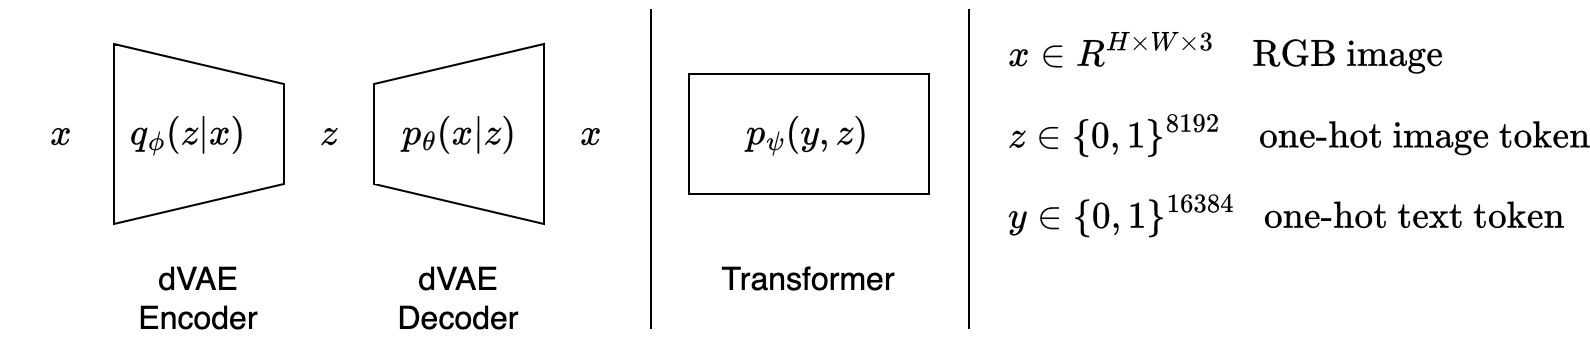
\includegraphics[width=0.9\linewidth]{dalle_components}
		\caption{DALL-E components}
		\label{fig:dallecomponents}
	\end{figure}

	With its multiple vocabularies, DALL-E has more components compared to GPT-2. \autoref{fig:dallecomponents} shows DALL-E's three components:(1) an image encoder $q_\phi({z|x})$ to convert RGB images $x$ into a discrete tokens $z$; (2) an image decoder $p_\theta({x|z})$ to convert discrete image tokens $z$  back into RGB images $x$; (3) a transformers $p_{\psi}(y,z)$ trained to predict/generate both text $y$/image $z$ tokens.
	
	
	\begin{figure}[h]
		\centering
		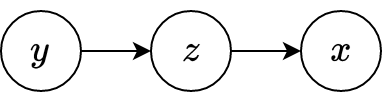
\includegraphics[width=0.3\linewidth]{dalle_graphical_model}
		\caption{DALL-E graphical moodel}
		\label{fig:dalle_graphical_model}
	\end{figure}

	%DALL-E's paper assumes a generative model $p_{\theta,\psi}(x,y,z)$ exists such that
	% over the RGB images $x$, image tokens $x$, and caption tokens $y$ 
	We believe DALL-E uses the graphical model depicted in~\autoref{fig:dalle_graphical_model}. Accordingly, the model's joint distribution is defined as follows
	\begin{equation}
			p_{\theta,\psi}(x,y,z) = p_{\theta}(x|y,z) p(z|y) p(y) =  p_{\theta}(x|y,z) p_{\psi}(y,z),
	\end{equation} 
	where $x, y, \text{and}\ z$ denote RGB images, text, and image-tokens, respectively. This yields the lower bound
	
	
	 %\begin{wrapfigure}{r}{0.5\textwidth}
	%	\begin{center}
	%		\includegraphics{factor_graph}
	%	\end{center}
	%	\caption{Birds}
	%\end{wrapfigure} this is bad.

	%  DALL-E introduces image-tokens $z$ so that training an auto-regressive model is a straight-forward. Concretely, RGB images are converted into a discrete space assuming vocabulary size $K_z=8192$. Along with the discrete space  $K_y=16384$ of captions $y$, the transformers  $p_{\psi}$ can be trained in a straight-forward manner. \autoref{fig:dallecomponents} shows the main components of DALL-E.
	
	
	

	
	% While it is natural to model both images $x$ and captions $y$, DALL-E's authors introduce image-tokens $z$. We believe $z$ have been introduced such that training an auto-regressive model is a straight-forward. It is worth noting that DALL-E comes from the same group/company that trains large language models (LLMs) such as ChatGPT. These LLMs are trained in an auto-regressive fashion. It is natural for the same group/company to train DALL-E, a text-to-image generator, in a same fashion, i.e., using auto regressive objective. While language can be easily discretized (e.g., characters/words/tokens), images are typically assumes to be "continuous" signals\footnote{This assumption has been questioned recently~\ref{}}. This continuous nature hinders 
	
	% & \eqparbox{C}{\hyperlink{thesentence}{Why Expectation (\ref{sec:integration})?}}
														 
	\begin{flalign}
				\ln p_{\theta,\psi}(x,y) &= \ln \int_{z} p_{\theta,\psi}(x,y,z)\,dz\\
													 &= \ln \int_{z} \frac{p_{\theta,\psi}(x,y,z)}{q_{\phi}(z|x)} q_{\phi}(z|x)\,dz\\
													 &= \ln \mathop{\EX}_{z\sim q_\phi(z|x)}\left[{\frac{p_{\theta,\psi}(x,y,z)}{q_{\phi}(z|x)}}\right] \\
													 &\ge \mathop{\EX}_{z\sim q_\phi(z|x)}\left[\ln\Bigl({\frac{p_{\theta,\psi}(x,y,z)}{q_{\phi}(z|x)}}\Bigr)\right] \\
													 &\ge \mathop{\EX}_{z\sim q_\phi(z|x)}\left[\ln{{p_{\theta,\psi}(x,y,z)}-\ln{q_{\phi}(z|x)}}\right] \\
													 %&\ge \mathop{\EX}_{z\sim %q_\phi(z|x)}\left[\ln{p_{\theta,\psi}(x,y,z)-\ln{q_{\phi}(z|x)}}\right] \\
													 &\ge \mathop{\EX}_{z\sim q_\phi(z|x)}\left[\ln{p_{\theta}(x|y,z) p_{\psi}(y,z)-\ln{q_{\phi}(z|x)}}\right] \\
													 &\ge \mathop{\EX}_{z\sim q_\phi(z|x)}\left[\ln{p_{\theta}(x|y,z) + \ln p_{\psi}(y,z)-\ln{q_{\phi}(z|x)}}\right]. \label{eq:dalle_i}
	\end{flalign}
	
	Now,~\autoref{eq:dalle_i} is missing the $D_{KL}$ term from~\autoref{eq:dall_e_eq}. Indeed,~\autoref{eq:dalle_i} has two terms $p_{\psi}(y,z)$ and $q_{\phi}(z|x)$, but these represent incompatible distributions. Concretely, $q_{\phi}(z|x)$ represents a univariate discrete distribution over the image tokens $z$, while $p_{\psi}(y,z)$ represents a multivariate (joint) discrete distribution over the joint image $z$ and text $y$ tokens as illustrated in~\autoref{fig:one_two_distributions}. Basically, it makes no sense to reduce the distance (Kullback-Leibler divergence) between these distributions.
	
		\begin{figure}[h]
		\centering
		\begin{subfigure}{0.45\linewidth}
			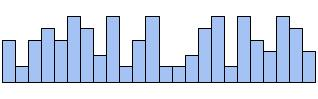
\includegraphics[width=\linewidth]{1D_dist.jpg}
			%\caption{Yellow color}
			%\label{fig:subfigA}
		\end{subfigure}
		\hfill
		\begin{subfigure}{0.45\linewidth}
			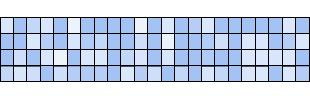
\includegraphics[width=\linewidth]{2D_dist.jpg}
			%\caption{Red color}
			%\label{fig:subfigB}
		\end{subfigure}
		\caption{(Left) A Toy univariate distribution over the image vocabulary $q_{\phi}(z|x)$. (Right) A Toy multivariate distribution over the joint image $z$ and text $y$ vocabularies $p_{\psi}(y,z)$.}
		\label{fig:one_two_distributions}
	\end{figure}
	
	To bring the $D_{KL}(\textcolor{blue}{q_\phi(y,z|x)}, \textcolor{red}{p_\psi(y,z)})$ term, we should convert the univariate $q_{\phi}(z|x)$ into a multivariate $q_{\phi}(y,z|x)$. Accordingly, we introduce $q_{\phi}(y|x)$ as follows
	


\begin{flalign}
	\ln p_{\theta,\psi}(x,y) &\ge \mathop{\EX}_{z\sim q_\phi(z|x)}\left[\ln{p_{\theta}(x|y,z) + \ln p_{\psi}(y,z)-\ln{q_{\phi}(z|x)} -\ln{q_{\phi}(y|x)} +\ln{q_{\phi}(y|x)} }\right] \\
	&\ge \mathop{\EX}_{z\sim q_\phi(z|x)}\left[\ln{p_{\theta}(x|y,z) + \ln p_{\psi}(y,z)-\ln{q_{\phi}(z|x)q_{\phi}(y|x)} +\ln{q_{\phi}(y|x)} }\right].
\end{flalign}

It is important to note that the dAVE encoder $q_{\phi}$ is trained to convert RGB images $x$ into a discrete image tokens $z$. Thus, the probability distribution over text tokens $q_{\phi}(y|x)$ is independent of both the dAVE encoder's parameter $\phi$ and input $x$,~\ie $q_{\phi}(z|x)q_{\phi}(y|x)=q_{\phi}(y,z|x)$



%follows a discrete distribution $\mathcal{U}$ uniformly distributed over $K_y=16384$ possible values,~\ie text tokens. The uniform distribution  $\mathcal{U}$ is assumed because this is the prior 


\begin{flalign}
	\ln p_{\theta,\psi}(x,y) &\ge \mathop{\EX}_{z\sim q_\phi(z|x)}\left[\ln{p_{\theta}(x|y,z) + \ln p_{\psi}(y,z)-\ln{q_{\phi}(y,z|x)} +\ln{q_{\phi}(y|x)} }\right] \\
	&\ge \mathop{\EX}_{z\sim q_\phi(z|x)}\left[\ln{p_{\theta}(x|y,z) - D_{KL}(\textcolor{blue}{q_\phi(y,z|x)}, \textcolor{red}{p_\psi(y,z)}) +\ln{q_{\phi}(y|x)} }\right] \label{eq:dalle_ii}.
\end{flalign}

Since $q_{\phi}(y|x)$ is independent of both $\phi$ and $x$, the term $q_{\phi}(y|x)$ follows the probability mass function of the BPE-encode learned by Sennrich~\etal~\cite{sennrich2015neural}. So, $\mathop{\EX}_{z\sim q_\phi(z|x)}\left[\ln{q_{\phi}(y|x)}\right]$ is a constant positive value that we can drop from~\autoref{eq:dalle_ii}. This leads to 

\begin{flalign}
	\ln p_{\theta,\psi}(x,y) &\ge \mathop{\EX}_{z\sim q_\phi(z|x)}\left[\ln{p_{\theta}(x|y,z) - \beta D_{KL}(\textcolor{blue}{q_\phi(y,z|x)}, \textcolor{red}{p_\psi(y,z)}) }\right], 
\end{flalign}

\noindent where the bound only holds for $\beta = 1$. In practice, Ramesh~\etal~\cite{ramesh2021zero} found that $\beta = 6.6$ promotes better codebook usage and ultimately leads to a smaller reconstruction error at the end of training \citep[cf.][\S 2.1]{ramesh2021zero}.



%	\hypertarget{thesentence}{\subsubsection{Integration \& Expectation}\label{sec:integration}}
%	Hello World



	%Maximizing likelihood is equivalent to minimizing KL divergence~\cite{ramesh2021zero}
	% https://www.youtube.com/watch?v=bWSkyZVSn_c
	
	{\small
		\bibliographystyle{ieee_fullname}
		\bibliography{dall_e_references}
	}
\end{document}